% thesis.tex
%
% This file is root file for an example thesis written using the
% University of Wisconsin-Madison LaTeX Style file.
%
% It is provided without warranty on an AS IS basis.


%=====================================================================
% Document Style
%=====================================================================
% Choose only one of the following document classes:
%
% for a 12 Point UW PhD Thesis without Margin Check
\documentclass[a4paper,12pt,twoside]{book}
%
% for a 10 Point UW PhD Thesis with Margin Check
%\documentclass[10pt,margincheck]{withesis}
%
% The margincheck option flags lines which overflow their hbox with a black
%  box at the end of the line.  This usually (but not always) indicates a
%  margin violation on the right margin.  Left margin violations aren't
%  indicated and if the margin violation is large enough, there isn't room
%  for the black box to be visiable.  
%
% This option can be also used in conjunction with the msthesis option.
%
% or for a 12 Point UW Masters Thesis
%\documentclass[12pt,msthesis]{withesis}
%
% or for a 10 Point UW Masters Thesis
%\documentclass[10pt,msthesis]{withesis}
%
% The msthesis option changes the page margins from 1" all around
% (the PhD format) to 1.25" left and 1" remaining margins (MS format).
% The defaults for degree and thesis are changed to be MS and thesis.
% These defaults can be overridden if the margins for the MS thesis
% are desired for other documents.

% To include optional packages, use the \usepackage command.
%  The package epsfig is used to bring in the Encapsulated PostScript
%    figures into the document.
%  The package times is used to change the fonts to Times Roman; however
%    because the times typewriter font looks odd, the original LaTeX
%    Computer Modern font is kept for the typewriter font using
%      \renewcommand{\ttdefault}{cmtt}
%    Note that Times Roman is a PostScript font and therefore, the document
%    cannot be correctly viewed from the *.dvi file.  It should be converted
%    to a *.ps file first and then viewed with a PostScript previewer...
\usepackage{epsfig}
\usepackage{graphicx}
\usepackage{url}
\usepackage{times}
\usepackage{datetime}
\renewcommand{\ttdefault}{cmtt}

\begin{document}

\bibliographystyle{plain}

\newcommand{\degree}[1]{\gdef\@degree{#1}}
\newcommand{\masterthesis}{\gdef\@doctype{A Master Thesis}}
\newcommand{\department}[1]{\gdef\@department{(#1)}}

\def\advisortitle#1{\gdef\@advisortitle{#1}}
\def\advisorname#1{\gdef\@advisorname{#1}}
\gdef\@advisortitle{Professor}
\gdef\@advisorname{Default Professor}

%=============================================================================
% COPYRIGHTPAGE
%=============================================================================
% The copyright must do the following:
% - start a new page with no number
% - place the copyright text centered at the bottom.
%=============================================================================
\def\copyrightpage{
  \newpage
  \thispagestyle{empty}    % No page number
  \addtocounter{page}{-1}
  \chapter*{}            % Required for \vfill to work
  \begin{center}
   \vfill
   \copyright\ Copyright by \actualauthor\ \date\\
   All Rights Reserved
  \end{center}}

\newcommand{\twoskip}{1.5}
\newcommand{\doublespace}
  {\renewcommand{\baselinestretch}{\twoskip}\Large\normalsize}

% prelude.tex
%   - titlepage
%   - dedication
%   - acknowledgments
%   - table of contents, list of tables and list of figures
%   - nomenclature
%   - abstract
%============================================================================


\clearpage\pagenumbering{gobble}  % This makes the page numbers Roman (i, ii, etc)



% TITLE PAGE
%   - define \title{} \author{} \date{}
\newcommand{\actualtitle}{Zimbra 8 High Availability on Ubuntu 12.04}
\title{\actualtitle}
\newcommand{\actualauthor}{Adri\'an Gibanel L\'opez}
\author{\actualauthor}
\date{2013}
%   - The default degree is ``Doctor of Philosophy''
%     (unless the document style msthesis is specified
%      and then the default degree is ``Master of Science'')
%     Degree can be changed using the command \degree{}
\degree{M\`aster en Enginyeria de Programari Lliure}
%   - The default is dissertation, unless the document style
%     msthesis was specified in which case it becomes thesis.
%     If msthesis is specified for the MS margins, you can
%     still have a dissertation if you specify \disseration
%\disseration
%   - for a masters project report, specify \project
%\project
%   - for a preliminary report, specify \prelim
%\prelim
%   - for a masters thesis, specify \thesis
\masterthesis
%   - The default department is ``Electrical Engineering''
%     The department can be changed using the command \department{}
\department{Dept. d'Informatica i Enginyeria Industrial}
%   - once the above are defined, use \maketitle to generate the titlepage
\advisorname{Josep Maria Rib\'o Balust}
\advisortitle{Professor}
\newdateformat{udlthesisdate}{\monthname[\THEMONTH] \THEYEAR}

% Title - BEGIN
\let\textquotedbl="
\pagestyle{empty}~

~

~

\begin{center}
{\LARGE \title{}}
\par\end{center}{\LARGE \par}

~
\begin{center}

\includegraphics[scale=0.4]{img/udl}
\par\end{center}
~

~

\begin{center}
{\large Universitat de Lleida}
\par\end{center}{\large \par}

\begin{center}
{\large Escola Polit\`ecnica Superior}
\par\end{center}{\large \par}

\begin{center}
{\large M\`aster en Enginyeria de Programari Lliure}
\par\end{center}{\large \par}

%\begin{center}
%{\large Dept. d'Informatica i Enginyeria Industrial}
%\par\end{center}{\large \par}


~

~
\begin{center}
{\large Treball de final de m\`aster}
\par\end{center}{\large \par}


~
\begin{center}
{\large \textbf{Zimbra 8 High Availability on Ubuntu 12.04}}
\par\end{center}{\large \par}


~

~


\hfill {\large Autor/a: Adri\'an Gibanel L\'opez}
\par{\large \par}

~

\hfill {\large Director/s: Josep Maria Rib\'o Balust}
\par{\large \par}

~

\hfill {\large Setembre 2013}
\par{\large \par}

\newpage

Copyright (c) 2013 Adrian Gibanel Lopez.

Permission is granted to copy, distribute and/or modify this document

under the terms of the GNU Free Documentation License, Version 1.3

or any later version published by the Free Software Foundation;

with no Invariant Sections, no Front-Cover Texts, and no Back-Cover
Texts.

A copy of the license is included in the section entitled \textquotedbl{}GNU

Free Documentation License\textquotedbl{}.

\newpage


% Title - END

% DEDICATION
\newpage
\null\vfil
\begin{center}
To the bTactic crew
\end{center}
\par\vfil\newpage

% ACKNOWLEDGMENTS

\chapter*{ACKNOWLEDGMENTS}
%\doublespace
I acknowledge Richard M. Stallman for his personal commitment to the free software movement.
\par\newpage




% ABSTRACT

\section* {ABSTRACT}
             \thispagestyle{empty}
                  \addtocounter{page}{-1}
                \begin{center}
                  {\bf\expandafter\uppercase\expandafter{\actualtitle}}\\
                  \vspace{12pt}
                  \actualauthor \\
                  \vspace{12pt}
                  Under the supervision of Professor Josep Maria Rib\'o Balust\\
                  At the Universitat de Lleida
                \end{center}

% abstract.tex
%
% This file has the abstract for the withesis style documentation
%
% Eric Benedict, Aug 2000
%
% It is provided without warranty on an AS IS basis.

\noindent       % Don't indent this paragraph.
The purpose of this master thesis is to design and test the setup of a Zimbra 8 Open Source Edition (OSE) High Availability System (HA) in Ubuntu 12.04.


\vspace*{0.5em}
\noindent       % Don't indent this paragraph.
A HA system has been proposed and tested in a laboratory environment. Its setup has been documented in its all length.

\vspace*{0.5em}
\noindent       % Don't indent this paragraph.
The master thesis shows that thanks to some minor modifications to Zimbra OSE core and thanks to freely available Open Source HA software one can achieve a HA Zimbra OSE system.

\vspace*{0.5em}
\noindent       % Don't indent this paragraph.
The proposed HA Zimbra OSE system can be improved in many ways and the author suggests several ways of doing so.

\pagestyle{headings}

% CONTENTS, TABLES, FIGURES
\tableofcontents
%\listoftables
\listoffigures
\newpage

\clearpage\pagenumbering{arabic} % This makes the page numbers Arabic (1, 2, etc)

% Problem description


\chapter{Introducing Zimbra High Availability}
This thesis was written to reflect the state of the art in High Availability methods for Zimbra Open Source Edition.  

\section {High Availability}
High availability is a system design approach and associated service implementation that ensures that a prearranged level of operational performance will be met during a contractual measurement period.

One of the most common high availability examples are web servers. Two web servers share the same information thanks to a shared storage. If one of the web servers fails to serve pages the other server can reclaim its primary role and shot the other node in the head (stonith) so that it can serve pages instead of the original primary node. The amount of time since the detection of the first server failure to its reestablishment is denoted as downtime. A contract for High Availability might stipulate that in a month time web servers service might be in downtime status for no more than five minutes.

High Availability, or HA as it is abbreviated, refers to the availability of resources in a computer system, in the event of component failures in the system. This can be achieved in a variety of ways, either with custom and redundant hardware to ensure availability or with software solutions using off-the-shelf hardware components.

The former class of solutions provide a higher degree of availability, but are significantly more expensive than the latter. This has led to the popularity of the latter class, with almost all vendors of computer systems offering various HA products. Typically, these products endure single points of failure in the system. (\cite{TaskForceHA})

As an example for more expensive systems we can mention OVH.co.uk web hosting service which uses more than 1,000 servers not only for ensuring high availability but also for dealing with high loads of visitor's queries. SQL servers seem to achieve high availability by using several RAID-1 (mirror) hard disks.

These HA systems usually ensure that a prearranged level of operational performance will be met during a contractual measurement period. (\cite{WikipediaHA})

High availability systems typically operate 24x7 and usually require built-in redundancy to minimize the risk of downtime due to hardware and/or telecommunication failures. 

Availability can be measured relative to "100\% operational" or "never failing." A widely-held but difficult-to-achieve standard of availability for a system or product is known as "five 9s" (99.999 percent) availability. (\cite{BCMHA})

From now on high availability will be refered as HA.

\section {Vmware Zimbra OSE}
VMware Zimbra is a complete email, address book, calendar and tasks solution that can be accessed from the Zimbra Web Client, Zimbra Desktop offline client, Outlook and a variety of other standards-based email clients and mobile devices. It can be deployed as a traditional binary install on Linux, or as a software virtual appliance, commonly referred to as Zimbra appliance.

Among the Zimbra Collaboration Server (ZCS) versions this thesis will approach the ZCS Open Source Edition also known as Zimbra OSE.

Vmware Zimbra OSE will be referred most of the times as Zimbra.

For more information about Vmware Zimbra you can visit: \cite{ZimbraLearn}.

\section {Vmware Zimbra OSE High Availability}
Zimbra OSE High Availability is a project which attempts to attain HA to each one of the Zimbra Collaboration Server components so that the risk of downtime due to hardware and/or telecommunication failures is minimized. High availability is usually implemented using High Availability software aimed at Gnu/Linux originally which is adapted to the Zimbra OSE setup.


\section{\label{sec:history}History}

Prior documentation about Zimbra High Availability was written with Zimbra 6 version in mind which is devoted to work (among others) in Ubuntu 8.04 64 bit. That documentation was based on Gnu/Linux High Availability software (heartbeat) which is no longer used for High Availability purposes nowadays.

To the best of the author's knowledge there is no updated documentation on how to setup this system.

On September 13th, 2012 Vmware announced Zimbra 8 which could be run in Ubuntu 12.04 (\cite{VmwareZimbra8Announce}).

\section {Main thesis topic}
The main topic of this thesis is: \\
\textit{Design and test the setup of a Zimbra 8 High Availability System in Ubuntu 12.04 and write a detailed report of this setup procedure.}

\section {Chosen technologies and solution}
We have decided to use the following proved open source HA technologies:\\ Corosync, Distributed Replicated Block Device (DRBD), OCF, and Pacemaker.

Corosync is a software meant to synchronize configuration files. Synchronize configuration files in a cluster is essential because all the cluster members have to share the same information and knowledge of the other cluster members. DRBD allows us to share a common storage between hosts as if a network RAID-1 hard disk it was. Finally, in order to setup and manage the whole cluster we will use Pacemaker cluster which uses OCF scripts as Cluster control scripts.

The reason for using these technologies is because they are the best well known and most used open source HA technologies. They have supersesed old technologies like heartbeat which we mentioned in \textbf{section {\ref{sec:history} History}}.

A set of virtual machines will be used to setup Zimbra 8 and Ubuntu 12.04 HA system. The neccessary steps to carry out this setup are: Setup network in both hosts, setup DRBD, initial Pacemaker setup, corosync installation, pacemaker installation, corosync setup, startup script disabling, DRBD script boot disabling, Pacemaker final setup, Pacemaker case of use tests.

This report describes in detail the setup procedure of each of these steps.

\section {Notation remarks}
Zimbra will be run in two \textit{servers} in our solution. These servers will be refered to as \textit{virtual servers} when we take the point of view of Virtualbox or virtualization point of view as in section \textbf {\ref{sec:virtualbox-implementation} Virtualbox implementation}.

When the HA system will be described these same servers will be refered to as \textit{nodes} as this is the way most HA software refer to their own cluster machines.

\section {Structure of the document}

Chapter 2 explains the high availability system that will be tested through the thesis.

Chapters 3 to 12 explain the detailed setup procedure of each element that constitutes the final system: \textit{\ref{chap:ha-schema} - High availability schema},
\textit{\ref{chap:operating-system-installation} - Operating System installation},
\textit{\ref{chap:network-setup} - Network setup},
\textit{\ref{chap:zimbra-installation} - Zimbra installation},
\textit{\ref{chap:drbd-setup} - DRBD Setup},
\textit{\ref{chap:zimbra-drbd-startup-script-disabling} - Zimbra and DRBD Startup Script Disabling},
\textit{\ref{chap:corosync-setup} - Corosync Setup},
\textit{\ref{chap:zimbra-ocf} - Zimbra OCF Resource Agent development},
and
\textit{\ref{chap:pacemaker-setup} - Pacemaker Setup}.
Final system is a Zimbra OSE High Availability system with two servers.

We learn how to manage our new High Availability system thanks to the \textit{\ref{chap:ha-system-management} - High Availability System Management} chapter.

Finally both conclusions and some of the ways this thesis can be improved are described in \textit{\ref{chap:conclusions-and-future-work}} chapter.


% HA Schema


\chapter{High availability schema}
\label{chap:ha-schema}
This chapter explains the high availability system that will be tested through the Thesis. 

\section {Purpose}
The proposed HA system is an Active/passive configuration. An Active/passive cluster provides a fully redundant instance of each node, which is only brought online when its associated primary node fails (\cite{HAClusterNodeConfigurations}).

In our case, the primary node will act as the active server and it will provide Zimbra services such as web server, smtp, imap, etc. The secondary node will be idle just waiting for the primary node to fail and bring Zimbra services online when that event happens. In addition the secondary node also mirrors Zimbra data partition in the background thanks to DRBD.

\section {Main schema}
There are two servers which we will be named as the primary one and the secondary one. They are linked by means of two connections: The service and the communication link.

The service link is the main network interface which is connected via a normal switch. It will serve content to the final users. The communication link, which is used for the cluster management and synchronization is done via a crossover cable.

We can see the main schema, where we have added two final clients at figure \ref{fig:main-schema}.

\begin{figure}
  \centering
    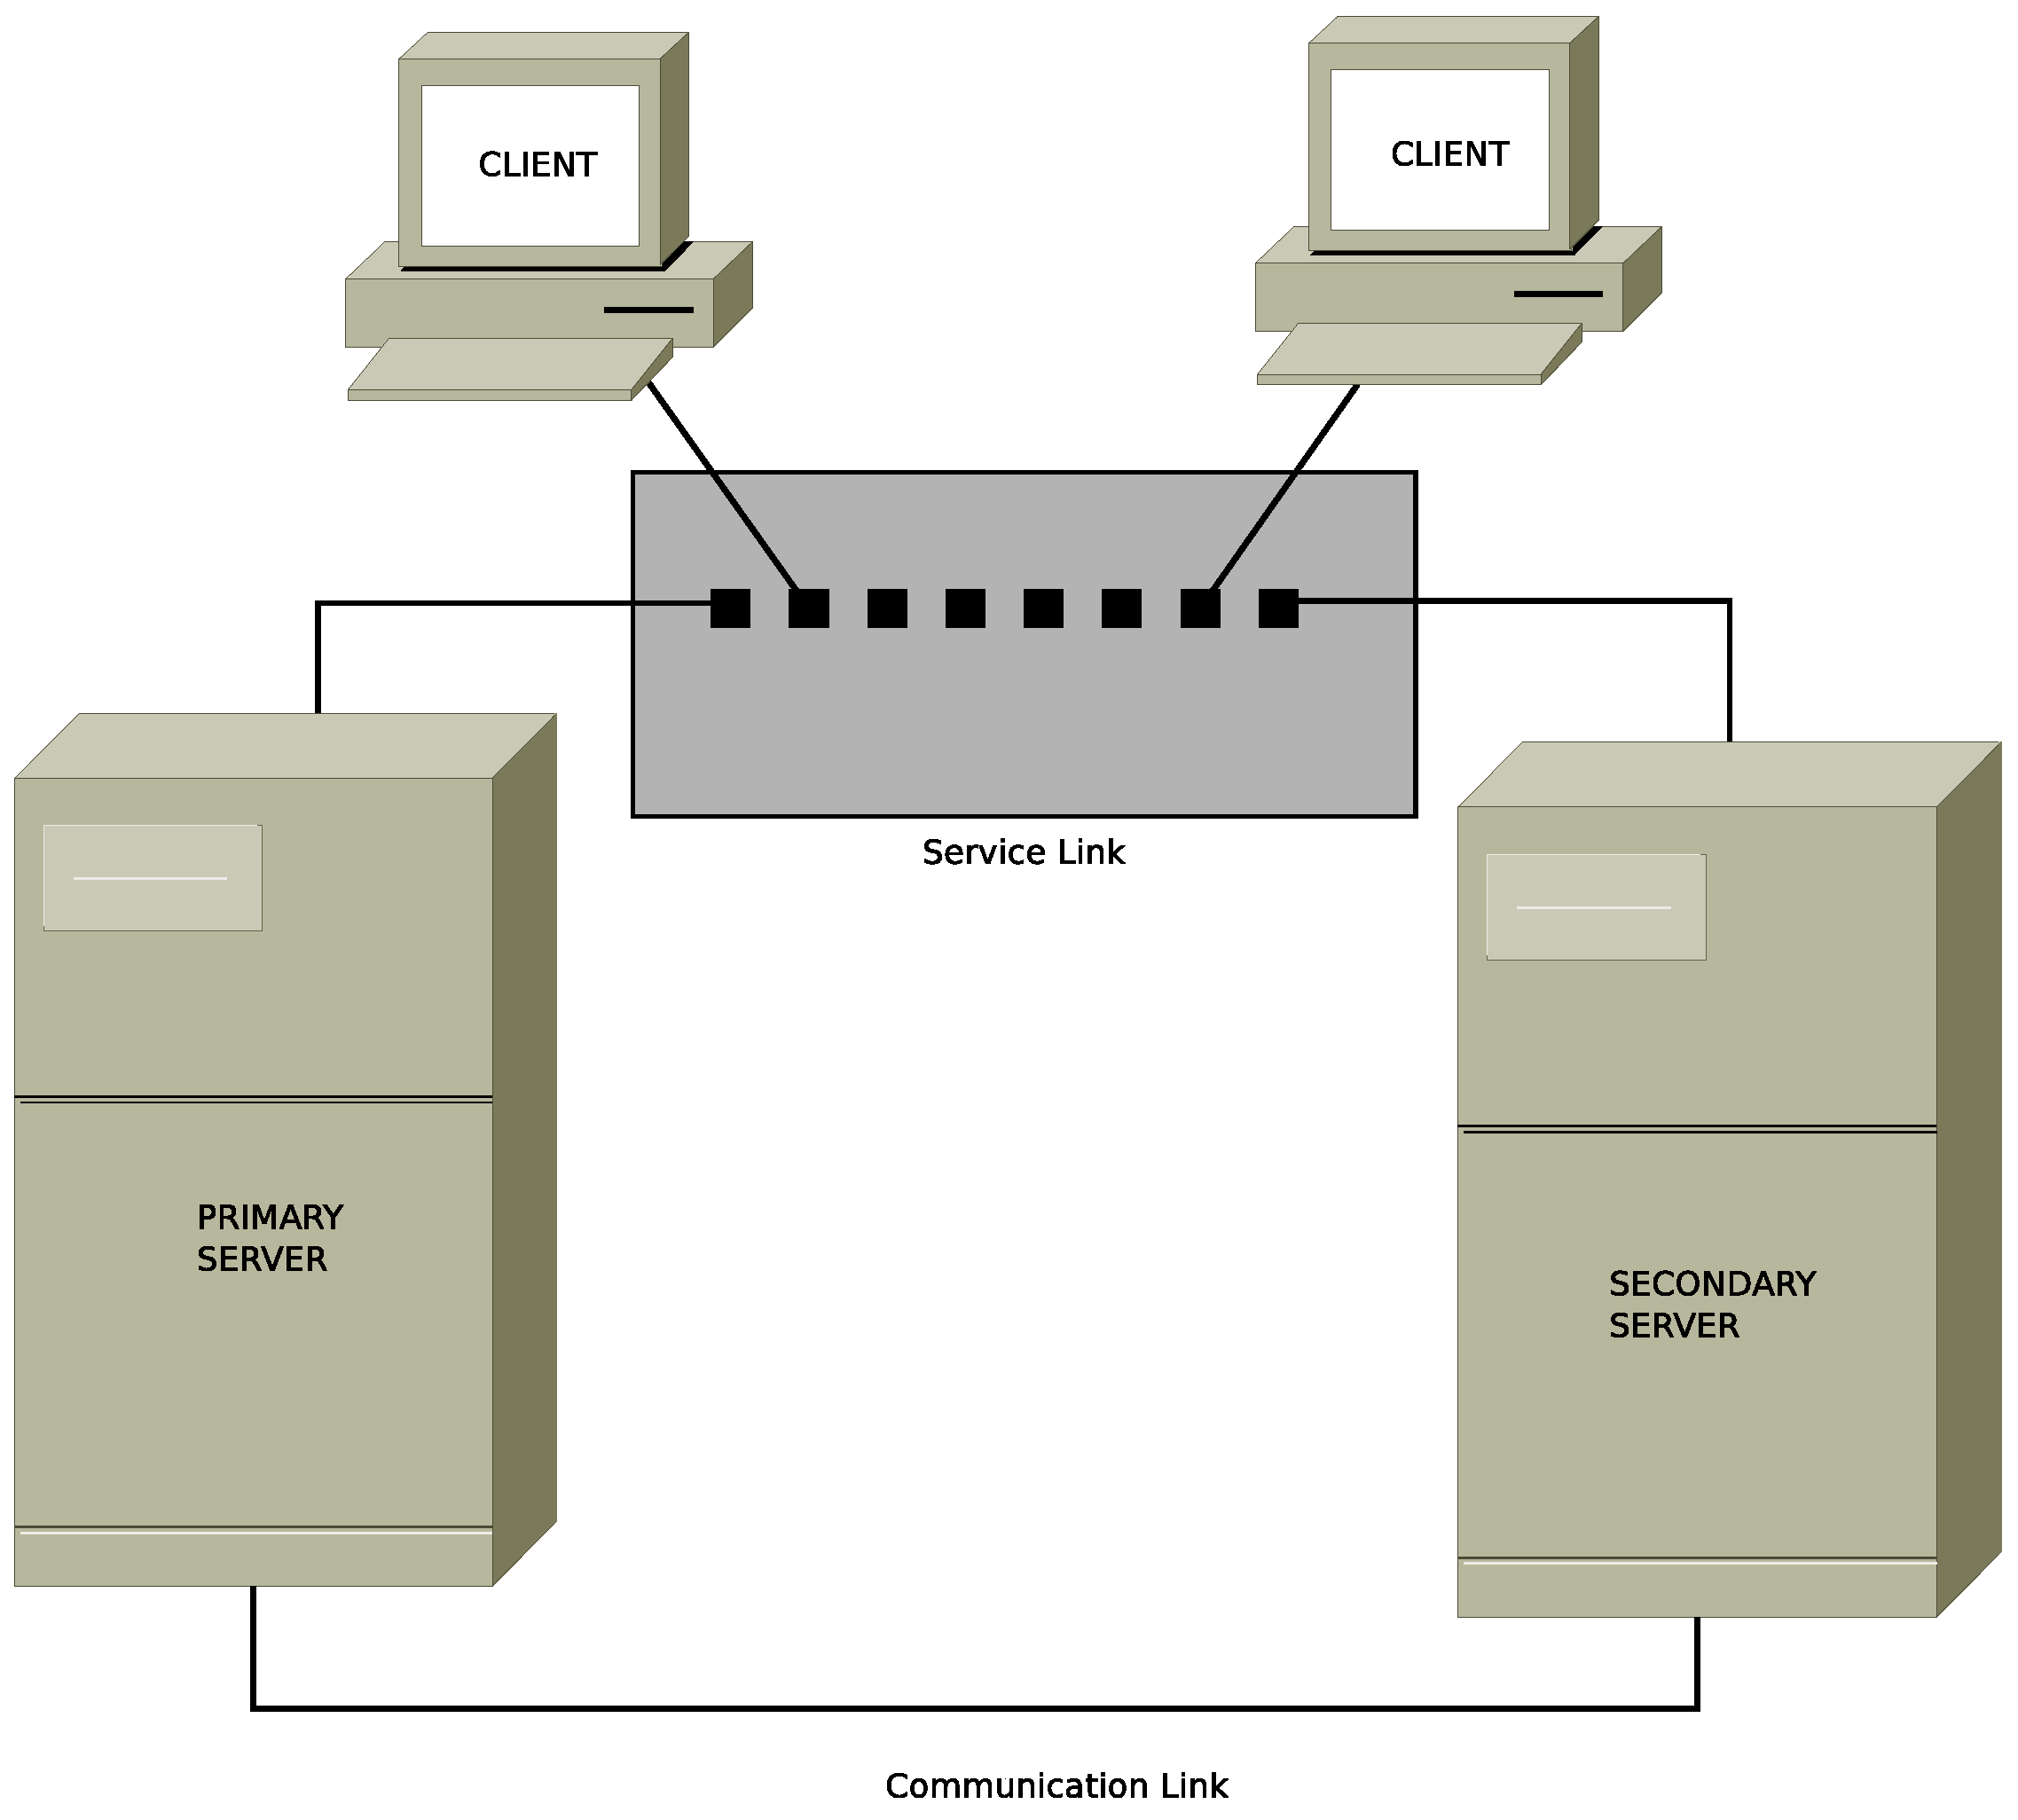
\includegraphics[width=0.8\textwidth]{img/ha_main_schema.eps}
  \caption{High Availability main schema}
  \label{fig:main-schema}
\end{figure}

\section {Primary server}
\subsection {Specifications}
The primary server specifications are as follow:
\begin{itemize}
  \item RAM: 4 GB
  \item Hard disk: 100 GB
  \item Processor: 2 x 2,40 Ghz
\end{itemize}

\section {Secondary server}
\subsection {Specifications}
The primary server specifications are as follow:
\begin{itemize}
  \item RAM: 4 GB
  \item Hard disk: 100 GB
  \item Processor: 2 x 2,40 Ghz
\end{itemize}

\section {\label{sec:virtualbox-implementation}Virtualbox implementation}
\subsection {Introduction}
Although in production environments High Availability systems are implemented in Physical servers or highly optimized virtualized servers, we are going to use Oracle VM Virtualbox software to emulate the described system. This section summarizes how to create both virtual machines and link them.

\subsection {\label{subsec:primary-virtual-machine-creation}Primary Virtual Machine creation}
We click on \textit{Machine} menu and select \textit{New} option. The Create Virtual Machine wizard will appear.

\subsubsection {Name and operating system}
\begin{itemize}
  \item Name: PrimaryZimbraHA
  \item Type: Linux
  \item Ubuntu (64 bit)
\end{itemize}

\subsubsection {Memory size}
Zimbra needs: 2048 MB as a minimum.
\subsubsection {Hard drive}
We select \textit{Create a virtual hard drive now}, \textit{Virtualbox Disk Image} as the hard drive file type, Dynamically allocated (so that the hard drive file only uses space as it fills up).

We leave the default File location and select hard disk size as 110 GB which is quite bigger than the strictly needed for our HA system.

\subsection {\label{subsec:service-link-primary}Service link network on Primary Virtual Machine}
We select \textit{PrimaryZimbraHA} virtual machine and click on \textit{Machine} menu and then in \textit{Settings} option. We will make sure we are in \textit{Network} section.

We will use default \textit{Adapter 1} for service link. We are going to summarize its setup:
\begin{itemize}
  \item Attached to: \textit{Internal Network}
  \item Name: ZimbraHAService
\end{itemize}

Finally we click on OK for saving changes.

\subsubsection {Secondary Virtual Machine creation}
In order to create secondary virtual machine we can either repeat the same steps as in \textbf{\ref{subsec:primary-virtual-machine-creation} Primary Virtual Machine creation}. Or we can make a linked clonation of the original machine. We will describe the latter option.

We select PrimaryZimbraHA virtual machine and then in \textit{Machine} menu we select \textit{Clone} option.

\textbf{New machine name}
\begin{itemize}
  \item New machine name: SecondaryZimbraHA
  \item Reinitialize the MAC address of all network cards: Checked
\end{itemize}

We select \textit{Linked clone} as Clone type.

Finally we click on \textit{Clone} button so that cloning is performed.

\subsection {Service link network on Secondary Virtual Machine}
As we did in subsection \textbf{\ref{subsec:service-link-primary} Service link network on Primary Virtual Machine} we select \textit{SecondaryZimbraHA} virtual machine and click on \textit{Machine} menu and then in \textit{Settings} option. We will make sure we are in \textit{Network} section.

We will use default \textit{Adapter 1} for service link. We are going to summarize its setup:
\begin{itemize}
  \item Attached to: \textit{Internal Network}
  \item Name: \textit{ZimbraHAService}
\end{itemize}

If we have cloned the virtual machine settings might be correct by default.

Finally we click on OK for saving changes.

\subsection {Communication link}
For both PrimaryZimbraHA and SecondaryZimbraHA virtual machines we will perform a very similar operation than the one done in subsection \textbf{\ref{subsec:service-link-primary} Service link network on Primary Virtual Machine}.

But now we make sure that we \textit{Adapter 2} is enabled as an \textit{Internal Network} which name is \textit{ZimbraHACommunication}.

\subsection {NAT link}
In order to make installation easier we will enable \textit{Adapter 3} in both virtual machines so that it can use the host Internet in order to fetch packages and perform post installation setup.

Similarly to subsection \textbf{\ref{subsec:service-link-primary} Service link network on Primary Virtual Machine} we make sure that \textit{Adapter 3} is enabled and that it's attached to NAT.

\subsection {Email client Virtual Machine}
A Virtual Machine whose only purpose is to test HA from a service link point of view might be added if needed. We're not to cover the installation and its setup here. We will just mention its network setup is similar to PrimaryZimbraHA and SecondaryZimbraHA but removing the second interface which serves for communication link and that, of course, doesn't make sense in an Email client VM.
% Operating System installation


\chapter{Operating System installation}
This chapter explains the Operating System installation.

\section {Introduction}
The reason why Ubuntu 12.04 in its 64bit mode is used is because is one of the official supported Operating System for Zimbra 8 versions. We denote an external DRBD metadata as DRBD-Meta-Disk. We can understand it is an special partition that helps DRBD system to track changes between synchronised partitions between both primary and secondary nodes. We can find a more accurate definition at Linbit site: \cite{LinbitDRBDInternals}.

\section {Ubuntu 12.04 64 bit minimal}
In order to track all the requisites and just install what the high availability system needs we will use an Ubuntu minimal disk for installation. These disks can be downloaded from \cite{UbuntuMinimalDisk}.

The used download was: \textit{Ubuntu 12.04 "Precise Pangolin" Minimal CD} from the \textit{64-bit PC (amd64, x86\_64)} section. 

\section {TODO: steps1}
\section {Partitioning}
Both virtual machines will have the same partitioning scheme. Both virtual machines have two hard disks.
Assuming a 1.8 Terabyte hard disk in order to setup DRBD-Meta-Disk there's enough with 59 megabytes. We will be on the safe side and setup it with a 150 megabytes size. In order to safe calculate other DRBD meta disk partitions we can check \cite{LinbitDRBDInternals}.

Hard Disk 1:
\begin{verbatim}
sda1 / 10GB ext4
sda2 DRBD-Meta-Disk 150MB ext4
sda3 (LVM Partition + Free space for LVM snapshots)
\end{verbatim}

sda3 contains a LVM's Volume Group named zimbra.
This Volume Group has a Logical Volume named zimbra also which doesn't ocuppy the full Volume Group space. The reason is that we reserver some space for snapshots when doing backups.

In our case we did:
\begin{verbatim}
VG zimbra: 1,8 TB

  LV zimbra: 1770 GB
  Free space: 30 GB
\end{verbatim}


Hard Disk 2:
\begin{verbatim}
sdb1 / 2 GB SWAP
\end{verbatim}

% Network Setup


\chapter{Network setup}
\label{chap:network-setup}
This chapter explains the network setup.

\section {Network schema}
We can just check the High Availability main schema (figure \ref{fig:main-schema}) where network has been already described. There are two networks. The service link is the main network interface for serving content to the final users. The communication link, which it's used for the cluster management and syncronisation is done via a crossover cable.

\section {VirtualBox Network Implementation}

In order to implement this Network schema in VirtualBox the service link will be setup by the first virtual network card in each virtual machine. Both of tese virtual network card will be setup in bridge mode so that an actual switch serve them. The communication link will be setup by the second virtual network card in each virtual machine connected to a VirtualBox private network, that means that they will be connected via a virtual switch given by Virtualbox which it's isolated from other networks.

TODO: Add VirtualBox Network figure.

\section {Network setup}

\subsection {Primary server}
\subsubsection {Service link}
Primary server's Service link network setup consists of a Class C configuration where the network card address is 192.168.1.201, as per being a Class C its netmask is 255.255.255.0 and thus its broadcast is 192.168.1.255. As a gateway it will be using the first network address in the network range which it's 192.168.1.1.

\begin{verbatim}
auto eth0
iface eth0 inet static
        address 192.168.1.201
        netmask 255.255.255.0
        broadcast 192.168.1.255
        gateway 192.168.1.1
\end{verbatim}

\subsubsection {Communication link}
Primary server's Communication link network setup consists of a Class C configuration where the network card address is 10.0.2.201, as per being a Class C its netmask is 255.255.255.0 and thus its broadcast is 10.0.2.255. As a gateway it will be using the first network address in the network range which it's 10.0.2.1.

\begin{verbatim}
auto eth0
iface eth0 inet static
        address 10.0.2.201
        netmask 255.255.255.0
        broadcast 10.0.2.255
        gateway 10.0.2.1
\end{verbatim}
\subsection {Secondary server}
\subsubsection {Service link}
Secondary server's Service link network setup consists of a Class C configuration where the network card address is 192.168.1.202, as per being a Class C its netmask is 255.255.255.0 and thus its broadcast is 192.168.1.255. As a gateway it will be using the first network address in the network range which it's 192.168.1.1.

\begin{verbatim}
auto eth0
iface eth0 inet static
        address 192.168.1.202
        netmask 255.255.255.0
        broadcast 192.168.1.255
        gateway 192.168.1.1
\end{verbatim}

\subsubsection {Communication link}
Secondary server's Communication link network setup consists of a Class C configuration where the network card address is 10.0.2.202, as per being a Class C its netmask is 255.255.255.0 and thus its broadcast is 10.0.2.255. As a gateway it will be using the first network address in the network range which it's 10.0.2.1.

\begin{verbatim}
auto eth0
iface eth0 inet static
        address 10.0.2.202
        netmask 255.255.255.0
        broadcast 10.0.2.255
        gateway 10.0.2.1
\end{verbatim}

\section {Firewall}

TODO: Describe firewall. Ports that have been left opened.



% Zimbra installation


\chapter{Zimbra installation}
\label{chap:zimbra-installation}
This chapter explains the Zimbra OSE installation.

\section {Zimbra 8.0.4 for Ubuntu 12.04}
Zimbra 8.0.4 for Ubuntu 12.04 in form of a tar.gz file was downloaded from \cite{Zimbra8Download}.
Once downloaded is advised to check its md5sum. Finally we untar it and cd into the untarred directory.

\section {Install script launch}



% DRBD Setup


\chapter{DRBD Setup}
This chapter explains the DRBD Setup.

\section {Introduction}
DRBD is a system that let us mirror a block device via an assigned device. DRBD can be understood as network based raid-1 and it's used in high availability (HA) clusters (\cite{LinbitDRBDWhatIs}).
We're using DRBD to mirror the block device where Zimbra files will be stored on.

\section {Requirements}
We will install DRBD packages for the Ubuntu 12.04 system thanks to the following command:
\begin{verbatim}
sudo apt-get install drbd8-utils
\end{verbatim}
.



\section {DRBD Resource config}
\textbf{To be performed in both servers}.

We will backup main drbd configuration file:
\begin{verbatim}
cp /etc/drbd.conf /etc/drbd.conf.orig
\end{verbatim}
.

We then need to edit:
\begin{verbatim}
/etc/drbd.conf
\end{verbatim}
so that it has:
\begin{verbatim}
resource zimbradata {
  protocol C;
  incon-degr-cmd "halt -f";
  startup {
    degr-wfc-timeout 120; # 2 min
  }
  disk {
    on-io-error detach;
  }
  net {
  }
  syncer {
    rate 10M;
    group 1;
    al-extents 257;
  }
  on zhatest-01.dominio.com {
    device /dev/drbd0;
    disk /dev/zimbra/zimbra;
    address zhatest-01-comm-ip:7788;
    meta-disk /dev/sda2[0];
  }
  on zhatest-02.dominio.com {
    device /dev/drbd0;
    disk /dev/zimbra/zimbra;
    address zhatest-02-comm-ip:7788;
    meta-disk /dev/sda2[0];
  }
}
\end{verbatim}
.

TODO: Explain drbd.conf contents and what they mean more or less.

If we want to modify our drbd.conf to increase sync rate, synchronised devices or any other settings we can check documentation at \cite{LinbitDRBDdrbdconf}.

\section {Start DRBD module}
\textbf{To be performed in both servers}.
\begin{verbatim}
modprobe drbd
\end{verbatim}
.
\section {Metadata disk initialisation}
\textbf{To be performed in both servers}.
We make sure the metadata partition does not have any prior metadata signature.
\begin{verbatim}
dd if=/dev/zero of=/dev/sda2 bs=1K count=100
\end{verbatim}
And we create the zimbradata metadata partition:
\begin{verbatim}
drbdadm create-md zimbradata
\end{verbatim}
.

\section {Primera sincronizaci\'on DRBD}
\textbf{To be performed in both servers}.
\begin{verbatim}
drbdadm up all
\end{verbatim}
where we shouldn't find any incorrect hostname errors.
TODO: Rewrite last line.

We will be asked about usage survey, we just reply that we don't want to participate by saying 'no'.

\textbf{To be performed in Primary server only}.
\begin{verbatim}
drbdadm -- --do-what-I-say primary all
drbdadm -- connect all
\end{verbatim}
.

If we happen to find a \textit{net-config disconnect first} error we can safely ignore it.

In order to check DRBD first synchronisation status we need to check /proc/drbd file with:
\begin{verbatim}
cat /proc/drbd
\end{verbatim}
which will output something like:
\begin{verbatim}
version: 0.7.20 (api:77/proto:74)
SVN Revision: 1743 build by <a href="mailto:phil@mescal">\
phil@mescal</a>, 2005-01-31 12:22:07
0: cs:SyncSource st:Primary/Secondary ld:Consistent
ns:13441632 nr:0 dw:0 dr:13467108 al:0 \
bm:2369 lo:0 pe:23 ua:226 ap:0
[==>..............] sync'ed: 3.1% (7000/7168)M
finish: 1:14:16 speed: 2,644 (2,204) K/sec
1: cs:Unconfigured
\end{verbatim}
.

We must wait for the process to finish in order to continue.







% Zimbra and DRBD Startup Script disabling


\chapter{Zimbra and DRBD startup scripts disabling}
\label{chap:zimbra-drbd-startup-script-disabling}
This chapter explains how to disable both Zimbra and DRBD startup scripts.

\section {Introduction}
We need to disable both default Zimbra and DRBD startup scripts because Pacemaker will be the responsible for starting and stopping both Zimbra and DRBD thanks to OCF scripts.

The explanation is that it is not safe to start Zimbra at boot because Zimbra needs its filesystem to be mounted. Filesystem needs DRBD to be loaded so that ZimbraData partition exists. All of this requirement are handle by pacemaker which is been setup for the task. The same reasoning applies to DRBD.

\section {Disable Zimbra startup scripts}
We just have to run \textbf{on both nodes}:
\begin{verbatim}
update-rc.d -f zimbra remove
\end{verbatim}

\section {Disable DRBD startup scripts}
We just have to run \textbf{on both nodes}:
\begin{verbatim}
update-rc.d -f drbd remove
\end{verbatim}

% COROSYNC Setup


\chapter{Corosync Setup}
This chapter explains the Corosync Setup.

\section {Corosync.conf}

The corosync.conf file on both computers it will be modified to use upnp so that we can use in non multicast environments. In order to use upnp we need to use a corosync version higher than 1.3 but that's not a problem because current version is higher than that.

\subsection {Primary server Corosync.conf}

We create the file:
\begin{verbatim}
/etc/corosync/corosync.conf
\end{verbatim}
which its contents will be:

TODO: Change zhatest-01-comm-ip and zhatest-02-comm-ip with actual ips
TODO: Explain a bit the settings in the file

\begin{verbatim}
# Please read the openais.conf.5 manual page

totem {
	version: 2

	# How long before declaring a token lost (ms)
	token: 5000

	# How many token retransmits before
	# forming a new configuration
	token_retransmits_before_loss_const: 20

	# How long to wait for join messages
	# in the membership protocol (ms)
	join: 1000

	# How long to wait for consensus to be achieved 
	# before starting a new round of
	# membership configuration (ms)
	consensus: 7500

	# Turn off the virtual synchrony filter
	vsftype: none

	# Number of messages that may be sent by one
	# processor on receipt of the token
	max_messages: 20

	# Limit generated nodeids to 31-bits
	# (positive signed integers)
	clear_node_high_bit: yes

	# Disable encryption
 	secauth: off

	# How many threads to use for encryption/decryption
 	threads: 0

	# Optionally assign a fixed node id (integer)
	 #nodeid: 1234


        rrp_mode: passive


interface {
		member {
			memberaddr: zhatest-01-comm-ip
		}
		member {
			memberaddr: zhatest-02-comm-ip
		}
        ringnumber: 0
        bindnetaddr: zhatest-01-comm-ip
        mcastport: 5405
        }
		transport: udpu
}
amf {
	mode: disabled
}

service {
 	# Load the Pacemaker Cluster Resource Manager
 	ver:       0
 	name:      pacemaker
}

aisexec {
        user:   root
        group:  root
}

logging {
        fileline: off
        to_stderr: yes
        to_logfile: no
        to_syslog: yes
	syslog_facility: daemon
        debug: off
        timestamp: on
   logger_subsys {
           subsys: AMF
           debug: off
tags: enter|leave|trace1|trace2|trace3|trace4|trace6
   }
}
\end{verbatim}

\subsection {Secondary server Corosync.conf}

We create the file:
\begin{verbatim}
/etc/corosync/corosync.conf
\end{verbatim}
which its contents will be:

TODO: Change zhatest-01-comm-ip and zhatest-02-comm-ip with actual ips
TODO: Explain a bit the settings in the file

\begin{verbatim}
# Please read the openais.conf.5 manual page

totem {
	version: 2

	# How long before declaring a token lost (ms)
	token: 5000

	# How many token retransmits before
	# forming a new configuration
	token_retransmits_before_loss_const: 20

	# How long to wait for join messages
	# in the membership protocol (ms)
	join: 1000

	# How long to wait for consensus to be achieved 
	# before starting a new round of
	# membership configuration (ms)
	consensus: 7500

	# Turn off the virtual synchrony filter
	vsftype: none

	# Number of messages that may be sent by one
	# processor on receipt of the token
	max_messages: 20

	# Limit generated nodeids to 31-bits
	# (positive signed integers)
	clear_node_high_bit: yes

	# Disable encryption
 	secauth: off

	# How many threads to use for encryption/decryption
 	threads: 0

	# Optionally assign a fixed node id (integer)
	 #nodeid: 1234


        rrp_mode: passive


interface {
		member {
			memberaddr: zhatest-01-comm-ip
		}
		member {
			memberaddr: zhatest-02-comm-ip
		}
        ringnumber: 0
        bindnetaddr: zhatest-02-comm-ip
        mcastport: 5405
        }
		transport: udpu
}
amf {
	mode: disabled
}

service {
 	# Load the Pacemaker Cluster Resource Manager
 	ver:       0
 	name:      pacemaker
}

aisexec {
        user:   root
        group:  root
}

logging {
        fileline: off
        to_stderr: yes
        to_logfile: no
        to_syslog: yes
	syslog_facility: daemon
        debug: off
        timestamp: on
   logger_subsys {
           subsys: AMF
           debug: off
tags: enter|leave|trace1|trace2|trace3|trace4|trace6
   }
}
\end{verbatim}

\section {Corosync's Authkey}
In the primary server we will create the file:
\begin{verbatim}
/etc/corosync/authkey
\end{verbatim}
thanks to running:
\begin{verbatim}
corosync-keygen
\end{verbatim}
.

In order to secure it we will need to run:
\begin{verbatim}
chown root:root /etc/corosync/authkey
chmod 400 /etc/corosync/authkey
\end{verbatim}
.

Once the file created we will copy the very same file to the secondary server in the same path as in primary server.

\section {Cfgtool}

In both servers we need to edit:
\begin{verbatim}
/etc/rc.local
\end{verbatim}
in order to add the line:
\begin{verbatim}
/usr/sbin/corosync-cfgtool -r
\end{verbatim}
just before the:
\begin{verbatim}
exit 0
\end{verbatim}
line.

TODO: That makes run corosync cfgtool at boot to inforce... WHAT?

\section {Corosync startup enabling}
In order to enable Corosync at boot we need to edit:
\begin{verbatim}
/etc/default/corosync
\end{verbatim}
file so that:
\begin{verbatim}
START=no
\end{verbatim}
line becomes:
\begin{verbatim}
START=yes
\end{verbatim}
.

\section {Corosync reboot and check}
In order to check Corosync startup we need to reboot the machine thanks to:
\begin{verbatim}
sync
shutdown -r now
\end{verbatim}
.

Once the machine has rebooted we can cluster status thanks to:
\begin{verbatim}
crm_mon
\end{verbatim}
.

TODO: Add some explanation on how to check if cluster is ok. What are the standard message for OK and KO errors.

% Corosync and Pacemaker installation

\chapter {Pacemaker setup}
\label{chap:pacemaker-setup}

This chapter explains the Pacemaker installation and setup.

\section {\label{sec:about-pacemaker}About Pacemaker}

Pacemaker is an Open Source, High Availability resource manager suitable for both small and large clusters (\cite{PacemakerWebpage}) which features:
\begin{itemize}
  \item Detection and recovery of machine and application-level failures
  \item Supports practically any redundancy configuration
  \item Supports both quorate and resource-driven clusters
  \item Configurable strategies for dealing with quorum loss (when multiple machines fail)
  \item Supports application startup/shutdown ordering, regardless machine(s) the applications are on
  \item Supports applications that must/must-not run on the same machine
  \item Supports applications which need to be active on multiple machines
  \item Supports applications with multiple modes (eg. master/slave)
  \item Provably correct response to any failure or cluster state. The cluster's response to any stimuli can be tested offline before the condition exists
\end{itemize}

Pacemaker let us manage the high availability cluster as a single system from anyone of the cluster nodes. In order to interact with each of the nodes it needs Corosync communication capabilities.


\section {Pacemaker installation}
\textbf{In both nodes} we just need to install Pacemaker packages for Ubuntu 12.04.

We need to issue this command:
\begin{verbatim}
apt-get install pacemaker
\end{verbatim}

We can safely ignore this warning:
\begin{verbatim}
Warning: The home dir /var/lib/heartbeat
 you specified already exists.
Adding system user `hacluster' (UID 105) ...
Adding new user `hacluster' (UID 105) with group `haclient' ...
The home directory `/var/lib/heartbeat' already exists.
 Not copying from `/etc/skel'.
adduser: Warning: The home directory `/var/lib/heartbeat'
 does not belong to the user you are currently creating.
Processing triggers for libc-bin ...
ldconfig deferred processing now taking place
\end{verbatim}
% Initial Pacemaker Setup

\section {About OCF Resource agents}
A resource agent is a standardized interface for a cluster resource. In translates a standard set of operations into steps specific to the resource or application, and interprets their results as success or failure(\cite{ResourceAgentsWiki}). An OCF resource agent is based on the Open Clustering Framework Resource Agent API specifications(\cite{OCFResourceAgentsWiki}). 

\section {bTactic Zimbra OCF installation}
\textbf{In both nodes} we need to obtain the Zimbra OCF script. Zimbra OCF script is found inside BtacticOCF tar.gz file (\cite{BtacticOCF}) which can be downloaded from BtacticOCF  tar.gz file (\cite{BtacticOrg}).

From the tar.gz we will use the zimbra script which we will copy into:
\begin{verbatim}
/usr/lib/ocf/resource.d/btactic
\end{verbatim}

We will use a temporary directory in order to use it:
\begin{verbatim}
mkdir /tmp/temp
cd /tmp/temp
\end{verbatim}
We download and extract it:
\begin{verbatim}
wget "http://www.btactic.org/btactic_ocf_0.0.2.tar.gz"
tar xzf btactic_ocf_0.0.2.tar.gz
\end{verbatim}
Make the btactic resource directory and copy zimbra file in there:
\begin{verbatim}
mkdir --parents /usr/lib/ocf/resource.d/btactic
cp zimbra /usr/lib/ocf/resource.d/btactic
\end{verbatim}
We finally make sure to give the script executable permissions:
\begin{verbatim}
chmod +x /usr/lib/ocf/resource.d/btactic/*
\end{verbatim}

% Pacemaker Final Setup

\section {\label{sec:pacemaker-final-setup}Pacemaker final setup}
As explained in \textit{section \ref{sec:about-pacemaker} About Pacemaker} Pacemaker is High Availability resource manager, here we will explain how our setup pretends to manage our two servers resources. These instructions should only be performed on \textbf{primary} node.

These are the main settings we define in our configuration:
\begin{itemize}
  \item Setup deletes prior configuration.
  \item DRBD, Filesystem mount and Zimbra Server are setup to work in the same server as they work as in a team.
  \item System stickiness is changed so that Zimbra Server resource is not moved from where it's running to avoid Zimbra innecessary downtimes.
  \item System are forced to be started in the right order. The right order is: DRBD, Filesystem mount, and Zimbra Server.
  \item We disable stonith in order to simplify the setup.
  \item Primary server will be the prefered server where resources need to be run.
\end{itemize}

TODO: Check if we define stickiness somewhere else and make a reference here.

TODO: Add an explanation on stonith on a new Improvements chapter and make here a reference to it.


We make sure that \textit{/tmp/zimbrapacemaker.config} file contents are:
\begin{verbatim}
configure
erase
node primary
node secondary
# Activate failover
property no-quorum-policy=ignore
# Disable stonith
property stonith-enabled=false
# Resource stickiness
rsc_defaults resource-stickiness=100
# Public ip fail over check
primitive ClusterIP ocf:heartbeat:IPaddr2 \
params nic=eth0 ip=192.168.77.203 \
cidr_netmask=24 \
broadcast=192.168.77.255 \
op monitor interval=30s
# Configure zimbra resource
primitive ZimbraServer ocf:btactic:zimbra op \
monitor interval=2min timeout="40s" \
op start interval="0" timeout="360s" \
op stop interval="0" timeout="360s"
# Prefered location: primary node
location prefer-primary-node \
ZimbraServer 50: primary
# Define DRBD ZimbraData
primitive ZimbraData ocf:linbit:drbd params \
drbd_resource=zimbradata op monitor \
role=Master interval=60s op monitor \
role=Slave interval=50s \
op start role=Master interval="0" timeout="240" \
op start role=Slave interval="0" timeout="240" \
op stop role=Master interval="0" timeout="100" \
op stop role=Slave interval="0" timeout="100"
# Define DRBD ZimbraData Clone
ms ZimbraDataClone ZimbraData meta \
master-max=1 master-node-max=1 \
clone-max=2 clone-node-max=1 notify=true
# Define ZimbraFS so that zimbra can use it
primitive ZimbraFS ocf:heartbeat:Filesystem \
params device="/dev/drbd/by-res/zimbradata" \
directory="/opt" fstype="ext4" \
op start interval="0" timeout="60s" \
op stop interval="0" timeout="60s"
group MyZimbra ZimbraFS ZimbraServer


# Everything in the same host
colocation everything-together \
inf: MyZimbra \
ZimbraDataClone:Master ClusterIP

# Everything ordered
order everything-ordered \
inf: \
ClusterIP \
ZimbraDataClone:promote MyZimbra
commit
\end{verbatim}

In order to apply the configuration we will run:
\begin{verbatim}
crm < /tmp/zimbrapacemaker.config
\end{verbatim}
.



Pacemaker configuration is not trivial. The main document from which the configuration file was adapted and written was Clusters from Scratch (\cite{ClustersFromScratch}).

TODO: Check if we need an order for normal ip ifconfig or whatever it's called.


% High Availability System Management


\chapter{High Availability System Management}
\label{chap:ha-system-management}
This chapter describes some common management tasks that can be used in the described High Availability System.

TODO: The described. Find a better rewording.

\section {Introduction}
Most of these examples have been extracted from Clusters From Scratch (\cite{ClustersFromScratch}) document . At Zimbra Forums Zimbra on Pacemaker + DRBD howto thread (\cite{ZForumsTaer}) we can find a Zimbra High Availability Howto (\cite{TaerHowtoHAZimbra8}) where we can find more every-day uses of Pacemaker examples.

The reason why we need these examples is that instead of managing a single server installation Zimbra server system now we need to manage a high availability system initially setup by Pacemaker. Some of the most useful management tasks will be described.

\section {DRBD Split Brain recovery}

Split brain is a situation where, due to temporary failure of all network links between cluster nodes, and possibly due to intervention by a cluster management software or human error, both nodes switched to the primary role while disconnected. This is a potentially harmful state, as it implies that modifications to the data might have been made on either node, without having been replicated to the peer. Thus, it is likely in this situation that two diverging sets of data have been created, which cannot be trivially merged (\cite{DrbdSplitBrain}).

This is an example of \textit{cat /proc/drbd} output:
\begin{verbatim}
version: 8.3.11 (api:88/proto:86-96)
srcversion: 93CE421BB73A731BDC72D8E 
 0: cs:WFConnection ro:Primary/Unknown ds:UpToDate/DUnknown C r-----
    ns:0 nr:0 dw:0 dr:1977 al:0 bm:0 lo:0 pe:0 ua:0 ap:0 ep:1 wo:f oos:153220
\end{verbatim}
where there is an split brain.

In order to fix it we can decide that primary node contents will prevail and that secondary node contents will be discarded. First of all we will need to stop the cluster on \textbf{both nodes} thanks to:
\begin{verbatim}
service corosync stop
\end{verbatim}
.

Then we need to start drbd service manually in \textbf{both nodes} thanks to:
\begin{verbatim}
service drbd start
\end{verbatim}

First of all \textbf{in secondary node} we will discard its data with:
\begin{verbatim}
drbdadm secondary zimbradata
drbdadm -- --discard-my-data connect zimbradata
\end{verbatim}
Then we will need to run \textbf{in primary node}:
\begin{verbatim}
drbdadm connect zimbradata
\end{verbatim}

Once we check that \textit{cat /proc/drbd} has a non split brain state like:
\begin{verbatim}
version: 8.3.11 (api:88/proto:86-96)
srcversion: 93CE421BB73A731BDC72D8E 
 0: cs:Connected ro:Primary/Secondary ds:UpToDate/UpToDate C r-----
    ns:5691029 nr:0 dw:0 dr:6002290 al:0 bm:367 lo:0 pe:0 ua:0 ap:0 ep:1 wo:f oos:0
\end{verbatim}
we can restart the cluster with running (\textbf{in both nodes}):
\begin{verbatim}
service drbd stop
service corosync start
\end{verbatim}
so that drbd is not handled manually and the cluster takes care of it.

\section {Host down simulation}
These commands simulate that a host is down by stopping both pacemaker and corosync services. We will run them only in the primary server. The secondary server is supposed to take control of the cluster system and start Zimbra.

\begin{verbatim}
service pacemaker stop
service corosync stop
\end{verbatim}

\section {Node recover}
In order to simulate a node recover we will start both pacemaker and corosync services in primary server:
\begin{verbatim}
service corosync start
service pacemaker start
\end{verbatim}

As per our our cluster system stickyness Zimbra service will stay in secondary server.


TODO: Cluster system is a synonym for High Availability cluster. Add it Prelude or similar chapter where definitions are done.

\section {Resources check}
In order to check the overall Cluster status we just run the cluster management monitor command:
\begin{verbatim}
crm_mon
\end{verbatim}

One example of crm\_mon output where the cluster has not problems at all is:
\begin{verbatim}
============
Last updated: Sun Sep  8 23:28:38 2013
Last change: Sun Sep  8 23:24:33 2013 via cibadmin on primary
Stack: openais
Current DC: secondary - partition with quorum
Version: 1.1.6-9971ebba4494012a93c03b40a2c58ec0eb60f50c
2 Nodes configured, 2 expected votes
5 Resources configured.
============

Online: [ secondary primary ]

 Master/Slave Set: ZimbraDataClone [ZimbraData]
     Masters: [ primary ]
     Slaves: [ secondary ]
 Resource Group: MySystem
     ClusterIP  (ocf::heartbeat:IPaddr2):       Started primary
 Resource Group: MyZimbra
     ZimbraFS   (ocf::heartbeat:Filesystem):    Started primary
     ZimbraServer       (ocf::btactic:zimbra):  Started primary
\end{verbatim}


TODO: Add an crm\_mon output as a listing and make a reference to it

\section {Move cluster resources temporarily}
In the case that we want to move \textit{temporarily} resources to primary server we should run:
\begin{verbatim}
crm resource move ZimbraServer primary
\end{verbatim}

\section {Disable cluster resources temporarily movement}
If we want to return Resource control to the cluster we can run:
\begin{verbatim}
crm resource unmove primary
\end{verbatim}
. In our setup, thanks to our defined stickiness the cluster won't perform any resource movement.

\section {Migration testing}
We can simulate the migration by declaring a node in standby. This way the standby node hardware can be fixed. We just have to run:
\begin{verbatim}
crm node standby
\end{verbatim}
in the affected node.

In order to check the migration status we can run:
\begin{verbatim}
crm_mon
\end{verbatim}
.

This is a crm\_mon output while node is migrating from primary node to secondary node:
\begin{verbatim}
============
Last updated: Sun Sep  8 23:33:41 2013
Last change: Sun Sep  8 23:31:50 2013 via crm_attribute on primary
Stack: openais
Current DC: secondary - partition with quorum
Version: 1.1.6-9971ebba4494012a93c03b40a2c58ec0eb60f50c
2 Nodes configured, 2 expected votes
5 Resources configured.
============

Node primary: standby
Online: [ secondary ]

 Master/Slave Set: ZimbraDataClone [ZimbraData]
     Masters: [ secondary ]
     Stopped: [ ZimbraData:1 ]
 Resource Group: MySystem
     ClusterIP  (ocf::heartbeat:IPaddr2):       Started secondary
 Resource Group: MyZimbra
     ZimbraFS   (ocf::heartbeat:Filesystem):    Started secondary
     ZimbraServer       (ocf::btactic:zimbra):  Stopped

\end{verbatim}
as we can see both ClusterIP and ZimbraFS have already started on secondary node and ZimbraServer is not started in secondary node yet.


Finally once we have fixed the hardware we can declare the node online again thanks to:
\begin{verbatim}
crm node online
\end{verbatim}
.

Once again in our setup, thanks to our defined stickiness the cluster won't perform any resource movement.

\section {Starting and stopping resources}
Sometimes, mainly for debugging purposes, is needed to start or stop cluster resources manually.

E.g. in order to start ZimbraFS resource we will issue:
\begin{verbatim}
crm resource start ZimbraFS
\end{verbatim}
In order to stop the same resource we will issue:
\begin{verbatim}
crm resource stop ZimbraFS
\end{verbatim}

TODO: Put references between all of these sections to explicify that there are linked one to another.


% Improvements


\chapter{Improvements}
\label{chap:improvements}
This chapter describes some of the improvements that can be applied to the described High Availability System. These improvements can be used in further research.

TODO: The described. Find a better rewording.

\section {OVH Datacentre network handling}
There have been some efforts from the bTactic team to handle OVH Datacentre networking thanks to three OCF scripts named: 
ClusterOVHFailover, ClusterHostRoute and ClusterDefaultRoute. These scripts make sense in setup that doesn't use Virtual Rack + RIPE but just normal servers connected via Internet only.

ClusterOVHFailover makes sure an OVH ip-fail-over is failed over from one machine to the another one. This way Zimbra Server is being served by the correct host.
ClusterHostRoute and ClusterDefaultRoute are meant to help to setup OVH networking for ip-fail-over which it's not covered by standard network setup found in  default Pacemaker package.

These scripts can be found inside BtacticOCF tar.gz file (\cite{BtacticOCF}) which can be downloaded from BtacticOCF  tar.gz file (\cite{BtacticOrg}). There were originally aimed as a complement for bTactic HA howto (\cite{BtacticZimbraHAHowto}).

\section {Fencing}
Fencing is the process of locking resources away from a node whose status is uncertain (\cite{LinuxHAFencing}). The default method of fencing in Pacemaker is using stonith. Stonith is a technique for NodeFencing, that means that the node (either primary or secondary server in our example) that it's supposed to have failed is \textit{shot in head} (\cite{LinuxHAStonith}). That makes sure that the node is actually dead.

In our described example we have disabled stonith. We can improve it by enabling it and using one of the available methods.

Once again bTactic team has developed an stonith script (or fence agent as known per Pacemaker) to make sure an OVH server doesn't use a shared resource. The failing node is rebooted into a Rescue mode which it's quite similar to booting a computer with a live cd that doesn't make any change to local hard disks. Fence agent name is: fence\_ovh.

This script is available as a Red Hat's fence-agents package since fence-agents package 4.0.2 release version (\cite{LinuxClusterML201307}).

\section {Mysql HA}
One of the Zimbra components is a Mysql database. This Mysql database can be excluded from DRBD syncing and can be setup as an active / active cluster.

This setup will offer a better handling of node failing because you would only loose last mysql queries. In the DRBD case you loose all the file changes that have not been stored into the files that compose actual Mysql database.

The only drawback for this improvement is that Zimbra OSE upgrades tend to be much more difficult when we want to preserve high availability.



     
%\include{figs}
%\include{bibs}

%\bibliography{refs}              % Make the bibliography

\begin{appendix}
\chapter{\label{cha:GFDL}GNU Free Documentation License}

GNU Free Documentation License

Version 1.3, 3 November 2008

Copyright (C) 2000, 2001, 2002, 2007, 2008 Free Software Foundation,
Inc. <http://fsf.org/> 

Everyone is permitted to copy and distribute verbatim copies of this
license document, but changing it is not allowed.

0. PREAMBLE

The purpose of this License is to make a manual, textbook, or other
functional and useful document \textquotedbl{}free\textquotedbl{}
in the sense of freedom: to assure everyone the effective freedom
to copy and redistribute it, with or without modifying it, either
commercially or noncommercially. Secondarily, this License preserves
for the author and publisher a way to get credit for their work, while
not being considered responsible for modifications made by others.

This License is a kind of \textquotedbl{}copyleft\textquotedbl{},
which means that derivative works of the document must themselves
be free in the same sense. It complements the GNU General Public License,
which is a copyleft license designed for free software.

We have designed this License in order to use it for manuals for free
software, because free software needs free documentation: a free program
should come with manuals providing the same freedoms that the software
does. But this License is not limited to software manuals; it can
be used for any textual work, regardless of subject matter or whether
it is published as a printed book. We recommend this License principally
for works whose purpose is instruction or reference.

1. APPLICABILITY AND DEFINITIONS

This License applies to any manual or other work, in any medium, that
contains a notice placed by the copyright holder saying it can be
distributed under the terms of this License. Such a notice grants
a world-wide, royalty-free license, unlimited in duration, to use
that work under the conditions stated herein. The \textquotedbl{}Document\textquotedbl{},
below, refers to any such manual or work. Any member of the public
is a licensee, and is addressed as \textquotedbl{}you\textquotedbl{}.
You accept the license if you copy, modify or distribute the work
in a way requiring permission under copyright law.

A \textquotedbl{}Modified Version\textquotedbl{} of the Document means
any work containing the Document or a portion of it, either copied
verbatim, or with modifications and/or translated into another language.

A \textquotedbl{}Secondary Section\textquotedbl{} is a named appendix
or a front-matter section of the Document that deals exclusively with
the relationship of the publishers or authors of the Document to the
Document's overall subject (or to related matters) and contains nothing
that could fall directly within that overall subject. (Thus, if the
Document is in part a textbook of mathematics, a Secondary Section
may not explain any mathematics.) The relationship could be a matter
of historical connection with the subject or with related matters,
or of legal, commercial, philosophical, ethical or political position
regarding them.

The \textquotedbl{}Invariant Sections\textquotedbl{} are certain Secondary
Sections whose titles are designated, as being those of Invariant
Sections, in the notice that says that the Document is released under
this License. If a section does not fit the above definition of Secondary
then it is not allowed to be designated as Invariant. The Document
may contain zero Invariant Sections. If the Document does not identify
any Invariant Sections then there are none.

The \textquotedbl{}Cover Texts\textquotedbl{} are certain short passages
of text that are listed, as Front-Cover Texts or Back-Cover Texts,
in the notice that says that the Document is released under this License.
A Front-Cover Text may be at most 5 words, and a Back-Cover Text may
be at most 25 words.

A \textquotedbl{}Transparent\textquotedbl{} copy of the Document means
a machine-readable copy, represented in a format whose specification
is available to the general public, that is suitable for revising
the document straightforwardly with generic text editors or (for images
composed of pixels) generic paint programs or (for drawings) some
widely available drawing editor, and that is suitable for input to
text formatters or for automatic translation to a variety of formats
suitable for input to text formatters. A copy made in an otherwise
Transparent file format whose markup, or absence of markup, has been
arranged to thwart or discourage subsequent modification by readers
is not Transparent. An image format is not Transparent if used for
any substantial amount of text. A copy that is not \textquotedbl{}Transparent\textquotedbl{}
is called \textquotedbl{}Opaque\textquotedbl{}.

Examples of suitable formats for Transparent copies include plain
ASCII without markup, Texinfo input format, LaTeX input format,
SGML or XML using a publicly available DTD, and standard-conforming
simple HTML, PostScript or PDF designed for human modification. Examples
of transparent image formats include PNG, XCF and JPG. Opaque formats
include proprietary formats that can be read and edited only by proprietary
word processors, SGML or XML for which the DTD and/or processing tools
are not generally available, and the machine-generated HTML, PostScript
or PDF produced by some word processors for output purposes only.

The \textquotedbl{}Title Page\textquotedbl{} means, for a printed
book, the title page itself, plus such following pages as are needed
to hold, legibly, the material this License requires to appear in
the title page. For works in formats which do not have any title page
as such, \textquotedbl{}Title Page\textquotedbl{} means the text near
the most prominent appearance of the work's title, preceding the beginning
of the body of the text.

The \textquotedbl{}publisher\textquotedbl{} means any person or entity
that distributes copies of the Document to the public.

A section \textquotedbl{}Entitled XYZ\textquotedbl{} means a named
subunit of the Document whose title either is precisely XYZ or contains
XYZ in parentheses following text that translates XYZ in another language.
(Here XYZ stands for a specific section name mentioned below, such
as \textquotedbl{}Acknowledgements\textquotedbl{}, \textquotedbl{}Dedications\textquotedbl{},
\textquotedbl{}Endorsements\textquotedbl{}, or \textquotedbl{}History\textquotedbl{}.)
To \textquotedbl{}Preserve the Title\textquotedbl{} of such a section
when you modify the Document means that it remains a section \textquotedbl{}Entitled
XYZ\textquotedbl{} according to this definition.

The Document may include Warranty Disclaimers next to the notice which
states that this License applies to the Document. These Warranty Disclaimers
are considered to be included by reference in this License, but only
as regards disclaiming warranties: any other implication that these
Warranty Disclaimers may have is void and has no effect on the meaning
of this License.

2. VERBATIM COPYING

You may copy and distribute the Document in any medium, either commercially
or noncommercially, provided that this License, the copyright notices,
and the license notice saying this License applies to the Document
are reproduced in all copies, and that you add no other conditions
whatsoever to those of this License. You may not use technical measures
to obstruct or control the reading or further copying of the copies
you make or distribute. However, you may accept compensation in exchange
for copies. If you distribute a large enough number of copies you
must also follow the conditions in section 3.

You may also lend copies, under the same conditions stated above,
and you may publicly display copies.

3. COPYING IN QUANTITY

If you publish printed copies (or copies in media that commonly have
printed covers) of the Document, numbering more than 100, and the
Document's license notice requires Cover Texts, you must enclose the
copies in covers that carry, clearly and legibly, all these Cover
Texts: Front-Cover Texts on the front cover, and Back-Cover Texts
on the back cover. Both covers must also clearly and legibly identify
you as the publisher of these copies. The front cover must present
the full title with all words of the title equally prominent and visible.
You may add other material on the covers in addition. Copying with
changes limited to the covers, as long as they preserve the title
of the Document and satisfy these conditions, can be treated as verbatim
copying in other respects.

If the required texts for either cover are too voluminous to fit legibly,
you should put the first ones listed (as many as fit reasonably) on
the actual cover, and continue the rest onto adjacent pages.

If you publish or distribute Opaque copies of the Document numbering
more than 100, you must either include a machine-readable Transparent
copy along with each Opaque copy, or state in or with each Opaque
copy a computer-network location from which the general network-using
public has access to download using public-standard network protocols
a complete Transparent copy of the Document, free of added material.
If you use the latter option, you must take reasonably prudent steps,
when you begin distribution of Opaque copies in quantity, to ensure
that this Transparent copy will remain thus accessible at the stated
location until at least one year after the last time you distribute
an Opaque copy (directly or through your agents or retailers) of that
edition to the public.

It is requested, but not required, that you contact the authors of
the Document well before redistributing any large number of copies,
to give them a chance to provide you with an updated version of the
Document.

4. MODIFICATIONS

You may copy and distribute a Modified Version of the Document under
the conditions of sections 2 and 3 above, provided that you release
the Modified Version under precisely this License, with the Modified
Version filling the role of the Document, thus licensing distribution
and modification of the Modified Version to whoever possesses a copy
of it. In addition, you must do these things in the Modified Version:

A. Use in the Title Page (and on the covers, if any) a title distinct
from that of the Document, and from those of previous versions (which
should, if there were any, be listed in the History section of the
Document). You may use the same title as a previous version if the
original publisher of that version gives permission. 

B. List on the Title Page, as authors, one or more persons or entities
responsible for authorship of the modifications in the Modified Version,
together with at least five of the principal authors of the Document
(all of its principal authors, if it has fewer than five), unless
they release you from this requirement. 

C. State on the Title page the name of the publisher of the Modified
Version, as the publisher. 

D. Preserve all the copyright notices of the Document. 

E. Add an appropriate copyright notice for your modifications adjacent
to the other copyright notices. 

F. Include, immediately after the copyright notices, a license notice
giving the public permission to use the Modified Version under the
terms of this License, in the form shown in the Addendum below. 

G. Preserve in that license notice the full lists of Invariant Sections
and required Cover Texts given in the Document's license notice. 

H. Include an unaltered copy of this License. 

I. Preserve the section Entitled \textquotedbl{}History\textquotedbl{},
Preserve its Title, and add to it an item stating at least the title,
year, new authors, and publisher of the Modified Version as given
on the Title Page. If there is no section Entitled \textquotedbl{}History\textquotedbl{}
in the Document, create one stating the title, year, authors, and
publisher of the Document as given on its Title Page, then add an
item describing the Modified Version as stated in the previous sentence. 

J. Preserve the network location, if any, given in the Document for
public access to a Transparent copy of the Document, and likewise
the network locations given in the Document for previous versions
it was based on. These may be placed in the \textquotedbl{}History\textquotedbl{}
section. You may omit a network location for a work that was published
at least four years before the Document itself, or if the original
publisher of the version it refers to gives permission. 

K. For any section Entitled \textquotedbl{}Acknowledgements\textquotedbl{}
or \textquotedbl{}Dedications\textquotedbl{}, Preserve the Title of
the section, and preserve in the section all the substance and tone
of each of the contributor acknowledgements and/or dedications given
therein. 

L. Preserve all the Invariant Sections of the Document, unaltered
in their text and in their titles. Section numbers or the equivalent
are not considered part of the section titles. 

M. Delete any section Entitled \textquotedbl{}Endorsements\textquotedbl{}.
Such a section may not be included in the Modified Version. 

N. Do not retitle any existing section to be Entitled \textquotedbl{}Endorsements\textquotedbl{}
or to conflict in title with any Invariant Section. 

O. Preserve any Warranty Disclaimers. 

If the Modified Version includes new front-matter sections or appendices
that qualify as Secondary Sections and contain no material copied
from the Document, you may at your option designate some or all of
these sections as invariant. To do this, add their titles to the list
of Invariant Sections in the Modified Version's license notice. These
titles must be distinct from any other section titles.

You may add a section Entitled \textquotedbl{}Endorsements\textquotedbl{},
provided it contains nothing but endorsements of your Modified Version
by various parties--for example, statements of peer review or that
the text has been approved by an organization as the authoritative
definition of a standard.

You may add a passage of up to five words as a Front-Cover Text, and
a passage of up to 25 words as a Back-Cover Text, to the end of the
list of Cover Texts in the Modified Version. Only one passage of Front-Cover
Text and one of Back-Cover Text may be added by (or through arrangements
made by) any one entity. If the Document already includes a cover
text for the same cover, previously added by you or by arrangement
made by the same entity you are acting on behalf of, you may not add
another; but you may replace the old one, on explicit permission from
the previous publisher that added the old one.

The author(s) and publisher(s) of the Document do not by this License
give permission to use their names for publicity for or to assert
or imply endorsement of any Modified Version.

5. COMBINING DOCUMENTS

You may combine the Document with other documents released under this
License, under the terms defined in section 4 above for modified versions,
provided that you include in the combination all of the Invariant
Sections of all of the original documents, unmodified, and list them
all as Invariant Sections of your combined work in its license notice,
and that you preserve all their Warranty Disclaimers.

The combined work need only contain one copy of this License, and
multiple identical Invariant Sections may be replaced with a single
copy. If there are multiple Invariant Sections with the same name
but different contents, make the title of each such section unique
by adding at the end of it, in parentheses, the name of the original
author or publisher of that section if known, or else a unique number.
Make the same adjustment to the section titles in the list of Invariant
Sections in the license notice of the combined work.

In the combination, you must combine any sections Entitled \textquotedbl{}History\textquotedbl{}
in the various original documents, forming one section Entitled \textquotedbl{}History\textquotedbl{};
likewise combine any sections Entitled \textquotedbl{}Acknowledgements\textquotedbl{},
and any sections Entitled \textquotedbl{}Dedications\textquotedbl{}.
You must delete all sections Entitled \textquotedbl{}Endorsements\textquotedbl{}.

6. COLLECTIONS OF DOCUMENTS

You may make a collection consisting of the Document and other documents
released under this License, and replace the individual copies of
this License in the various documents with a single copy that is included
in the collection, provided that you follow the rules of this License
for verbatim copying of each of the documents in all other respects.

You may extract a single document from such a collection, and distribute
it individually under this License, provided you insert a copy of
this License into the extracted document, and follow this License
in all other respects regarding verbatim copying of that document.

7. AGGREGATION WITH INDEPENDENT WORKS

A compilation of the Document or its derivatives with other separate
and independent documents or works, in or on a volume of a storage
or distribution medium, is called an \textquotedbl{}aggregate\textquotedbl{}
if the copyright resulting from the compilation is not used to limit
the legal rights of the compilation's users beyond what the individual
works permit. When the Document is included in an aggregate, this
License does not apply to the other works in the aggregate which are
not themselves derivative works of the Document.

If the Cover Text requirement of section 3 is applicable to these
copies of the Document, then if the Document is less than one half
of the entire aggregate, the Document's Cover Texts may be placed
on covers that bracket the Document within the aggregate, or the electronic
equivalent of covers if the Document is in electronic form. Otherwise
they must appear on printed covers that bracket the whole aggregate.

8. TRANSLATION

Translation is considered a kind of modification, so you may distribute
translations of the Document under the terms of section 4. Replacing
Invariant Sections with translations requires special permission from
their copyright holders, but you may include translations of some
or all Invariant Sections in addition to the original versions of
these Invariant Sections. You may include a translation of this License,
and all the license notices in the Document, and any Warranty Disclaimers,
provided that you also include the original English version of this
License and the original versions of those notices and disclaimers.
In case of a disagreement between the translation and the original
version of this License or a notice or disclaimer, the original version
will prevail.

If a section in the Document is Entitled \textquotedbl{}Acknowledgements\textquotedbl{},
\textquotedbl{}Dedications\textquotedbl{}, or \textquotedbl{}History\textquotedbl{},
the requirement (section 4) to Preserve its Title (section 1) will
typically require changing the actual title.

9. TERMINATION

You may not copy, modify, sublicense, or distribute the Document except
as expressly provided under this License. Any attempt otherwise to
copy, modify, sublicense, or distribute it is void, and will automatically
terminate your rights under this License.

However, if you cease all violation of this License, then your license
from a particular copyright holder is reinstated (a) provisionally,
unless and until the copyright holder explicitly and finally terminates
your license, and (b) permanently, if the copyright holder fails to
notify you of the violation by some reasonable means prior to 60 days
after the cessation.

Moreover, your license from a particular copyright holder is reinstated
permanently if the copyright holder notifies you of the violation
by some reasonable means, this is the first time you have received
notice of violation of this License (for any work) from that copyright
holder, and you cure the violation prior to 30 days after your receipt
of the notice.

Termination of your rights under this section does not terminate the
licenses of parties who have received copies or rights from you under
this License. If your rights have been terminated and not permanently
reinstated, receipt of a copy of some or all of the same material
does not give you any rights to use it.

10. FUTURE REVISIONS OF THIS LICENSE

The Free Software Foundation may publish new, revised versions of
the GNU Free Documentation License from time to time. Such new versions
will be similar in spirit to the present version, but may differ in
detail to address new problems or concerns. See http://www.gnu.org/copyleft/.

Each version of the License is given a distinguishing version number.
If the Document specifies that a particular numbered version of this
License \textquotedbl{}or any later version\textquotedbl{} applies
to it, you have the option of following the terms and conditions either
of that specified version or of any later version that has been published
(not as a draft) by the Free Software Foundation. If the Document
does not specify a version number of this License, you may choose
any version ever published (not as a draft) by the Free Software Foundation.
If the Document specifies that a proxy can decide which future versions
of this License can be used, that proxy's public statement of acceptance
of a version permanently authorizes you to choose that version for
the Document.

11. RELICENSING

\textquotedbl{}Massive Multiauthor Collaboration Site\textquotedbl{}
(or \textquotedbl{}MMC Site\textquotedbl{}) means any World Wide Web
server that publishes copyrightable works and also provides prominent
facilities for anybody to edit those works. A public wiki that anybody
can edit is an example of such a server. A \textquotedbl{}Massive
Multiauthor Collaboration\textquotedbl{} (or \textquotedbl{}MMC\textquotedbl{})
contained in the site means any set of copyrightable works thus published
on the MMC site.

\textquotedbl{}CC-BY-SA\textquotedbl{} means the Creative Commons
Attribution-Share Alike 3.0 license published by Creative Commons
Corporation, a not-for-profit corporation with a principal place of
business in San Francisco, California, as well as future copyleft
versions of that license published by that same organization.

\textquotedbl{}Incorporate\textquotedbl{} means to publish or republish
a Document, in whole or in part, as part of another Document.

An MMC is \textquotedbl{}eligible for relicensing\textquotedbl{} if
it is licensed under this License, and if all works that were first
published under this License somewhere other than this MMC, and subsequently
incorporated in whole or in part into the MMC, (1) had no cover texts
or invariant sections, and (2) were thus incorporated prior to November
1, 2008.

The operator of an MMC Site may republish an MMC contained in the
site under CC-BY-SA on the same site at any time before August 1,
2009, provided the MMC is eligible for relicensing.

ADDENDUM: How to use this License for your documents

To use this License in a document you have written, include a copy
of the License in the document and put the following copyright and
license notices just after the title page:

Copyright (c) YEAR YOUR NAME.

Permission is granted to copy, distribute and/or modify this document

under the terms of the GNU Free Documentation License, Version 1.3

or any later version published by the Free Software Foundation;

with no Invariant Sections, no Front-Cover Texts, and no Back-Cover
Texts.

A copy of the license is included in the section entitled \textquotedbl{}GNU

Free Documentation License\textquotedbl{}.

If you have Invariant Sections, Front-Cover Texts and Back-Cover Texts,
replace the \textquotedbl{}with...Texts.\textquotedbl{} line with
this:

with the Invariant Sections being LIST THEIR TITLES, with the

Front-Cover Texts being LIST, and with the Back-Cover Texts being
LIST.

If you have Invariant Sections without Cover Texts, or some other
combination of the three, merge those two alternatives to suit the
situation.

If your document contains nontrivial examples of program code, we
recommend releasing these examples in parallel under your choice of
free software license, such as the GNU General Public License, to
permit their use in free software. 

%\include{code}                   % Including computer code listings
%\include{bibref}                 % a BibTeX reference
%\include{math}                   % Complex Equations from the UW Math Department
%\include{acro}                   % A discussion on generating PDF files.
\end{appendix}

\begin{thebibliography}{1}

% problem-description

\bibitem[WIHA]{WikipediaHA} High Availability Wikipedia Article
\url{http://en.wikipedia.org/wiki/High_availability}. Last access 2013-08-20.

\bibitem[ATFC]{TaskForceHA} IEEE Task Force on Cluster Computing. archive.org capture from February 2011.
\url{http://web.archive.org/web/20110216113021/http://www.ieeetfcc.org/high-availability.html}. Last access 2013-08-20.

\bibitem[BCHA]{BCMHA} High Availability Bcmpedia definition
\url{http://www.bcmpedia.org/wiki/High_Availability}. Last access 2013-08-20.

\bibitem[ZLEA]{ZimbraLearn} Zimbra - Learn
\url{http://www.zimbra.com/learn/}. Last access 2013-08-20.

\bibitem[BZHA]{BtacticZimbraHAHowto} ZimbraOSE-Alta disponibilidad con DRBD con una ip-fail-over - 26 de agosto de 2012
\url{http://www.btactic.org/zimbra_ose_alta_disponibilidad_drbd_1_ipfailover.pdf}. Last access 2013-08-20

\bibitem[VWZ8]{VmwareZimbra8Announce} Zimbra Blog - Announcing The General Availability of Zimbra 8
\url{http://blog.zimbra.com/blog/archives/2012/09/announcing-the-general-availability-of-zimbra-8.html}. Last access 2013-08-20.

% operating-system-installation

\bibitem[UMIN]{UbuntuMinimalDisk} Ubuntu Community Help Wiki - Installation - MinimalCD
\url{https://help.ubuntu.com/community/Installation/MinimalCD}. Last access 2013-08-20.

\bibitem[LDIN]{LinbitDRBDInternals} LinBit DRBD version 8.4 Guide - Chapter 17 . DRBD Internals
\url{http://www.drbd.org/users-guide/ch-internals.html}. Last access 2013-08-20.

% zimbra-installation

\bibitem[VWZD]{Zimbra8Download} Zimbra - Open Source Edition Downloads
\url{http://www.zimbra.com/downloads/os-downloads.html}. Last access 2013-08-20.

\end{thebibliography}



%\include{vita}                  % Optional Vita, use \begin{vita} vita text \end{vita}
\end{document}
